\documentclass[tikz,border=4pt]{standalone}
\usepackage[T1]{fontenc}
\usepackage{lmodern}
\usetikzlibrary{arrows.meta}
\begin{document}
% Size of the compiler output (lines) for a rejected or warned defect; horizontal axis is logarithmic.
% x = 3.2 cm * log10(lines). Data, measured by the scripts on every run: 08_reprodutibilidade/logs/05_c_cpp_matrix.md
% (column "Diagnóstico em A": C M1, C++ M5, typed T3, T5 and T1) and 02_negative_matrix.md (InFlight -> Shutdown).
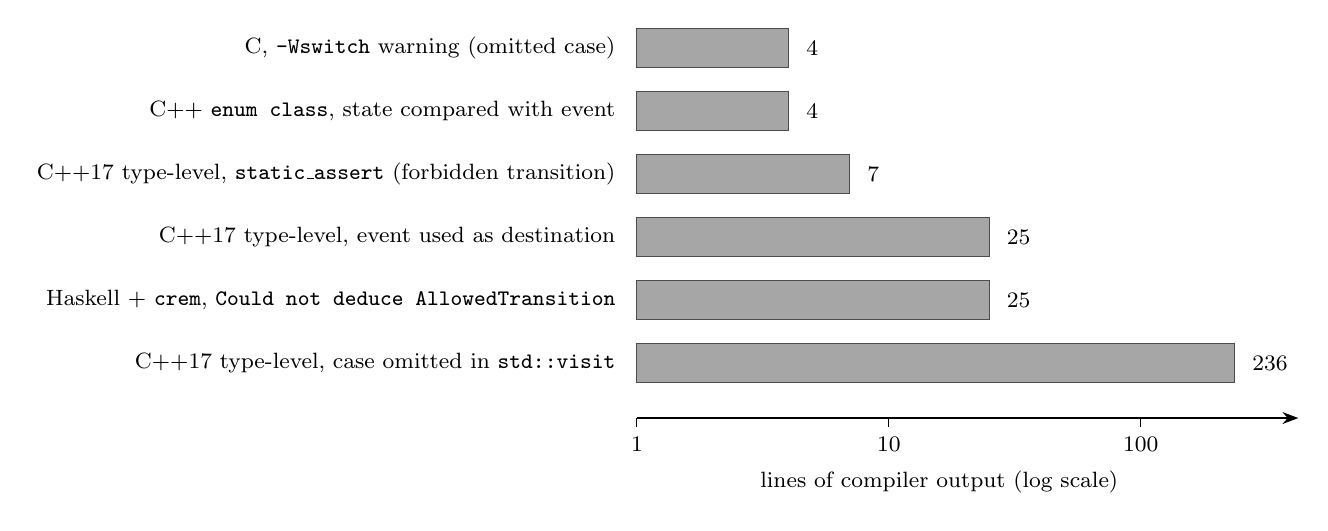
\begin{tikzpicture}[
    lab/.style={font=\footnotesize, anchor=east},
    val/.style={font=\footnotesize, anchor=west},
    bar/.style={fill=black!35, draw=black!70, line width=0.3pt}
]
\def\k{3.2}
\foreach \y/\n/\t in {
  0/4/{C, \texttt{-Wswitch} warning (omitted case)},
  -0.8/4/{C++ \texttt{enum class}, state compared with event},
  -1.6/7/{C++17 type-level, \texttt{static\_assert} (forbidden transition)},
  -2.4/25/{C++17 type-level, event used as destination},
  -3.2/25/{Haskell + \texttt{crem}, \texttt{Could not deduce AllowedTransition}},
  -4.0/236/{C++17 type-level, case omitted in \texttt{std::visit}}} {
  \pgfmathsetmacro{\w}{\k*log10(\n)}
  \fill[bar] (0,\y-0.25) rectangle (\w,\y+0.25);
  \node[lab] at (-0.15,\y) {\t};
  \node[val] at (\w+0.1,\y) {\n};
}
\draw[-{Stealth[length=2mm]}, thick] (0,-4.7) -- (\k*2.5+0.4,-4.7);
\foreach \x/\l in {1/1, 10/10, 100/100} {
  \pgfmathsetmacro{\px}{\k*log10(\x)}
  \draw (\px,-4.7) -- (\px,-4.82);
  \node[font=\footnotesize, anchor=north] at (\px,-4.82) {\l};
}
\node[font=\footnotesize, anchor=north] at (\k*1.2,-5.25) {lines of compiler output (log scale)};
\end{tikzpicture}
\end{document}
